\section{Simplex-Algorithmus}

\begin{enumerate}
\item \textbf{Vorbereitung:}
	\begin{itemize}
	\item \textbf{Lineares Programm (LP) in Ungleichungsform bringen:}\\
	$\boxed{\max\{\mathbf{c} \mathbf{x}, \mathbf{x}\in\mathbb{R}^n :\mathbf{Ax}\leq \mathbf{b}\}\\}$\quad(Alle Nebenbedingungen mit $\leq$ formulieren; $\mathbf{c}$ ist ein Zeilenvektor)
	\item \textbf{Erste zulässige Basisauswahl} $B=\begin{Bmatrix}\ldots\end{Bmatrix}$, für beliebigen Eckpunkt (Vertex) des Polyeders, \textbf{treffen:}\\
	Bei Vorgabe einer Ecke bilden die Ungleichungen welche diese Ecke definieren, die erste Basis.
	\end{itemize}
	
	\vspace{0.3cm}
	
\item \textbf{Algorithmus:}
	\begin{enumerate}
	\item \textbf{Basis bestimmen: } $\boxed{\mathbf{A}_B=\{\mathbf{A}\}_{B}}$\quad und \quad $\boxed{\mathbf{b}_{B}=\{\mathbf{b}\}_{B}}$\quad ($B_i$-te Zeilen aus \textbf{A} und \textbf{b} auswählen)\\
	\item Berechnung der \textbf{Basis-Inversen: }$\boxed{\overline{\mathbf{A}}=\mathbf{A}_B^{-1}}$\quad und der dazugehörigen \textbf{Basis-Lösung: }$\boxed{\mathbf{v}=\mathbf{\overline{A}}\cdot\mathbf{b}_B}$\\
	\item Berechnung der \textbf{''reduzierten Kosten''}: $\boxed{\mathbf{u}=\mathbf{c\overline{A}}}$
	\begin{itemize}
		\item $u_i<0$: Den ''negativsten'' Wert $u_j$ von $\mathbf{u}$ und die dazugehörige Spalte $\mathbf{\overline{a}}_j$ von $\mathbf{\overline{A}}$ bestimmen.\\
		(Wenn die $j$-te Zahl in $u$ der ''negativsten'' Zahl entspricht so ist die $j$-te Spalte in $\mathbf{\overline{A}}$ die dazugehörige Spalte). Behalte $j$ als Index der ursprünglichen Matrix $\mathbf{A}$!
		\item $u_i\geq 0$: Wenn $\mathbf{u}$ keine negativen Werte aufweist, wurde das Maximum der Zielfunktion gefunden:\\
		\textbf{Argument der Maximalstelle:} $\boxed{\mathbf{x^*}=\mathbf{v}}$\\
		\textbf{Maximalstelle:} 
		$\boxed{f(\mathbf{x^*})=\left\{
		  \begin{array}{ll}
		    \mathbf{c}\cdot\mathbf{v} & \text{Wenn anfängliches Problem eine Maximierung war}\\
		    -\mathbf{c}\cdot\mathbf{v}& \text{Wenn anfängliches Problem eine Minimierung war}
		  \end{array}
		\right.}$
	\end{itemize}
	\item \textbf{Richtungsvektor} für Bewegung auf Kante: $\boxed{\mathbf{d}=-\mathbf{\overline{A}}_j}$
	\item \textbf{Bewegung in Richtung von} $\mathbf{d}$ solange \textbf{alle} Nebenbedingungen erfüllt.\\
	
	$\boxed{\mathbf{A}(\mathbf{v}+\lambda\cdot \mathbf{d})\leq \mathbf{b}}\quad\Rightarrow\quad\lambda^*$\quad($\lambda^*$ ist der Maximalwert von $\lambda$ welcher alle Nebenbedingungen noch erfüllt.)\\
		
	Berechnung von $k$: $\lambda^* = \min\limits_k \left\{ \frac{b_i-\mathbf{a}^i\mathbf{v}}{\mathbf{a}^i\mathbf{d}}: i \in I, \mathbf{a}^i\mathbf{d} > 0\right\}$
		
	\begin{itemize}
		\item $0\leq\lambda^*<\infty$\qquad \textbf{Weiter mit (f):} Zielfunktion in Richtung $\mathbf{d}$ durch Bedingung $k$ beschränkt
		\item $\lambda^*\rightarrow\infty$\qquad\quad~ \textbf{Abbruch:} Zielfunktion wächst unbeschränkt in Richtung von $\mathbf{d}$
	\end{itemize}
	\item \textbf{Basistausch:} $B'(j)=k$ bzw. $B' = B - (\{j\} \cup \{k\})$\qquad $\boxed{\mathbf{v'}=\mathbf{v}+\lambda^*\cdot \mathbf{d}}$\quad (Die Basis an $j$-ter Stelle in B wird durch $k$ ersetzt)\\
	
	\textbf{Setze} $\boxed{B:=B'}$,\quad $\boxed{\mathbf{v}:=\mathbf{v'}}$ und \textbf{beginne bei Punkt (a)}
	\end{enumerate}
\end{enumerate}

\subsection{Beispiel:}
Das unten stehende LP-System soll mittels Simplexalgorithmus gelöst werden. Es soll im Punkt $V_0=\begin{bmatrix}0 & 1\end{bmatrix}$ begonnen werden.\\

\begin{minipage}[t]{0.66\textwidth}
	\begin{minipage}[t]{0.3\linewidth}
		\textbf{1.Durchlauf} \\
		$\max~~\{x_1-2x_2\}$\\
		$\begin{array}{ccc}
			x_1+x_2 & \leq & 2\\
			x_1 & \geq & 0\\
			x_2 & \leq & 1\\
			x_2 & \geq & -1\\
			
			
		\end{array}$
	\end{minipage}
	\hfill
	\begin{minipage}[t]{0.34\linewidth}
		\textbf{In Ungleichungsform:} \\
		$\max~~\{x_1-2x_2\}$\\
		$\begin{array}{ccc}
			x_1+x_2 & \leq & 2\\
			-x_1 & \leq & 0\\
			x_2 & \leq & 1\\
			-x_2 & \leq & 1\\
			
		\end{array}$
	\end{minipage}
	\hfill
	\begin{minipage}[t]{0.34\linewidth}
	\textbf{Matrizenschreibweise:}\\
	$c=\begin{bmatrix}
	1&-2
	\end{bmatrix}$\\
	$A=\begin{bmatrix}
	1  &  1 \\
	-1 &  0 \\
	 0 &  1 \\
	 0 & -1 
	\end{bmatrix}\quad 
	b=\begin{bmatrix}
	2\\
	0\\
	1\\
	1
	\end{bmatrix}$
	\end{minipage}\\
	\\
	
Die erste zulässige Basis: $B=\begin{Bmatrix}2&3\end{Bmatrix}\quad\Rightarrow\quad \mathbf{A_B}=\begin{bmatrix}-1&0\\0&1\end{bmatrix},\quad \mathbf{b_B}=\begin{bmatrix}0\\1\end{bmatrix}$

\subsubsection{Algorithmus}
 
\textbf{1.Durchlauf}
\begin{itemize}
\item[(a)] $\mathbf{A_B}=\{\mathbf{A}\}_{\mathbf{B}}=\begin{bmatrix}-1&0\\0&1\end{bmatrix}$\qquad $\mathbf{b}_\mathbf{B}=\{\mathbf{b}\}_{\mathbf{B}}=\begin{bmatrix}0\\1\end{bmatrix}$
\item[(b)] $\overline{\mathbf{A}}=\mathbf{A_B}^{-1}=\begin{bmatrix}-1&0\\0&1\end{bmatrix}^{-1}=\begin{bmatrix}-1&0\\0&1\end{bmatrix}\qquad
\mathbf{v}=\mathbf{\overline{A}}\cdot\mathbf{b_B}=\begin{bmatrix}0\\1\end{bmatrix}$


\end{itemize}
\end{minipage}
\hfill
\begin{minipage}[t]{0.30\textwidth}
\textbf{Zeichnung:}\\
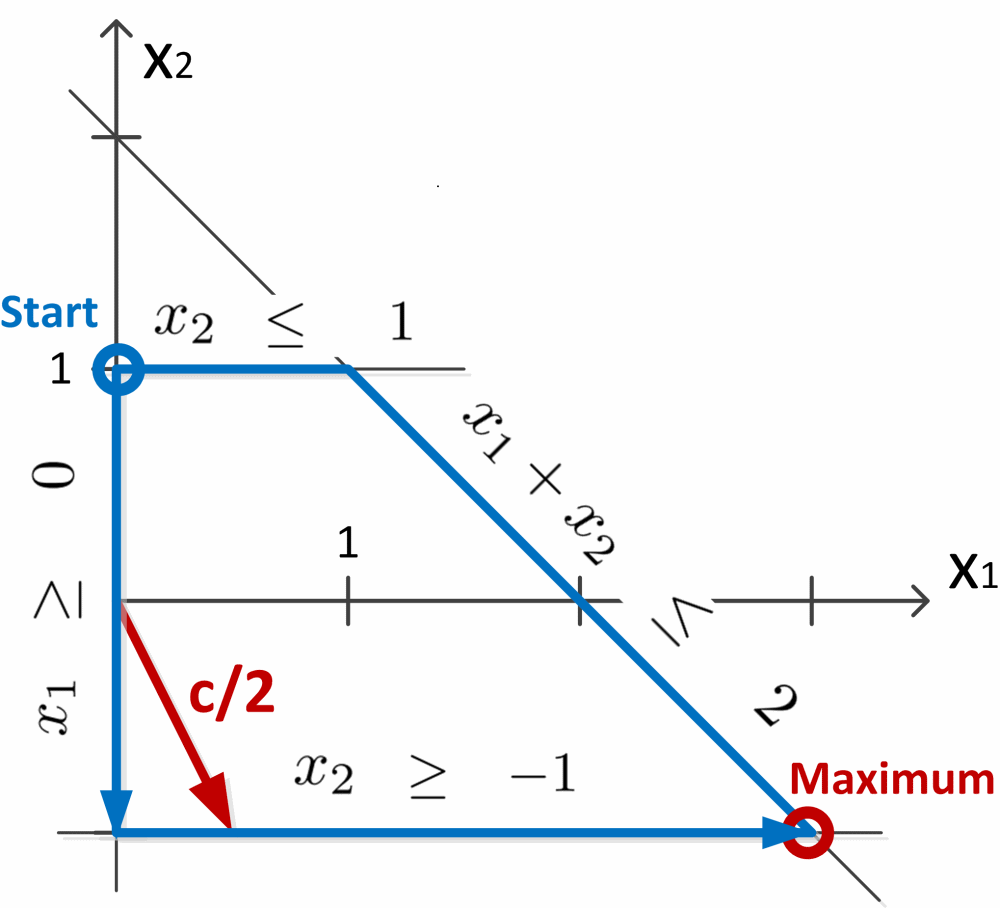
\includegraphics[width=\linewidth]{Content/Simplex/Polyeder.png} 
\end{minipage}
\begin{itemize}
	\item[(c)] $\mathbf{u}=\mathbf{c\overline{A}}=\begin{bmatrix}1&-2\end{bmatrix}\cdot\begin{bmatrix}-1&0\\0&1\end{bmatrix}=\begin{bmatrix}-1&-2\end{bmatrix}\quad\Rightarrow\quad \mathbf{\overline{a}}_j=\begin{bmatrix}0\\1\end{bmatrix}\qquad j=2$
	\item[(d)] $\mathbf{d}=-\mathbf{\overline{a}}_j=\begin{bmatrix}0\\-1\end{bmatrix}$ 
	\item[(e)] $\mathbf{A}(\mathbf{v}+\lambda\cdot \mathbf{d})\leq \mathbf{b}\quad\Rightarrow\quad\begin{bmatrix}
		1  &  1 \\
		-1 &  0 \\
		 0 &  1 \\
		 0 & -1 
		\end{bmatrix}\cdot\left(\begin{bmatrix}0\\1\end{bmatrix}+\lambda\cdot\begin{bmatrix}0\\-1\end{bmatrix}\right)\leq \begin{bmatrix}
			2\\
			0\\
			1\\
			1
			\end{bmatrix}\quad\Rightarrow\quad\begin{bmatrix}1\\0\\1\\-1\end{bmatrix}+
			\begin{bmatrix}-\lambda\\0\\-\lambda\\\lambda\end{bmatrix}\leq\begin{bmatrix}2\\0\\1\\1\end{bmatrix}\quad\Rightarrow\quad\lambda^*=2\qquad k=4$
	\item[(f)] $B'(j)=k\quad\Rightarrow\quad B'=\begin{Bmatrix}2&4\end{Bmatrix}\qquad \mathbf{v'}=\mathbf{v}+\lambda^*\cdot \mathbf{d}=\begin{bmatrix}0\\1\end{bmatrix}+2\cdot\begin{bmatrix}0\\-1\end{bmatrix}=\begin{bmatrix}0\\-1\end{bmatrix}$
\end{itemize}

\vspace{0.5cm}
\textbf{2.Durchlauf}
\begin{itemize}
	\item[(a)] $\mathbf{A_B}=\{\mathbf{A}\}_{\mathbf{B}}=\begin{bmatrix}-1&0\\0&-1\end{bmatrix}$\qquad $\mathbf{b}_\mathbf{B}=\{\mathbf{b}\}_{\mathbf{B}}=\begin{bmatrix}0\\1\end{bmatrix}$
	\item[(b)] $\overline{\mathbf{A}}=\mathbf{A_B}^{-1}=\begin{bmatrix}-1&0\\0&-1\end{bmatrix}^{-1}=\begin{bmatrix}-1&0\\0&-1\end{bmatrix}\qquad
	\mathbf{v}=\mathbf{\overline{A}}\cdot\mathbf{b_B}=\begin{bmatrix}0\\-1\end{bmatrix}$
	\item[(c)] $\mathbf{u}=\mathbf{c\overline{A}}=\begin{bmatrix}1&-2\end{bmatrix}\cdot\begin{bmatrix}-1&0\\0&-1\end{bmatrix}=\begin{bmatrix}-1&2\end{bmatrix}\quad\Rightarrow\quad \mathbf{\overline{a}}_j=\begin{bmatrix}-1\\0\end{bmatrix}\qquad j=1$
	\item[(d)] $\mathbf{d}=-\mathbf{\overline{a}}_j=\begin{bmatrix}1\\0\end{bmatrix}$ 
	\item[(e)] $\mathbf{A}(\mathbf{v}+\lambda\cdot \mathbf{d})\leq \mathbf{b}\quad\Rightarrow\quad\begin{bmatrix}
		1  &  1 \\
		-1 &  0 \\
		 0 &  1 \\
		 0 & -1 
		\end{bmatrix}\cdot\left(\begin{bmatrix}0\\-1\end{bmatrix}+\lambda\cdot\begin{bmatrix}1\\0\end{bmatrix}\right)\leq \begin{bmatrix}
			2\\
			0\\
			1\\
			1
			\end{bmatrix}\quad\Rightarrow\quad\begin{bmatrix}-1\\0\\-1\\1\end{bmatrix}+
			\begin{bmatrix}\lambda\\-\lambda\\0\\0\end{bmatrix}\leq\begin{bmatrix}2\\0\\1\\1\end{bmatrix}\quad\Rightarrow\quad\lambda^*=3\qquad k=1$
	\item[(f)] $B'(j)=k\quad\Rightarrow\quad B'=\begin{Bmatrix}1&4\end{Bmatrix}\qquad \mathbf{v'}=\mathbf{v}+\lambda^*\cdot \mathbf{d}=\begin{bmatrix}0\\-1\end{bmatrix}+3\cdot\begin{bmatrix}1\\0\end{bmatrix}=\begin{bmatrix}3\\-1\end{bmatrix}$
\end{itemize}

\vspace{0.5cm}
\textbf{3.Durchlauf}
\begin{itemize}
	\item[(a)] $\mathbf{A_B}=\{\mathbf{A}\}_{\mathbf{B}}=\begin{bmatrix}1&1\\0&-1\end{bmatrix}$\qquad $\mathbf{b}_\mathbf{B}=\{\mathbf{b}\}_{\mathbf{B}}=\begin{bmatrix}2\\1\end{bmatrix}$
	\item[(b)] $\overline{\mathbf{A}}=\mathbf{A_B}^{-1}=\begin{bmatrix}1&1\\0&-1\end{bmatrix}^{-1}=\begin{bmatrix}1&1\\0&-1\end{bmatrix}\qquad
	\mathbf{v}=\mathbf{\overline{A}}\cdot\mathbf{b_B}=\begin{bmatrix}3\\-1\end{bmatrix}$
	\item[(c)] $\mathbf{u}=\mathbf{c\overline{A}}=\begin{bmatrix}1&-2\end{bmatrix}\cdot\begin{bmatrix}1&1\\0&-1\end{bmatrix}=\begin{bmatrix}1&3\end{bmatrix}$\\
	\textbf{Argument der Maximalstelle:} $\mathbf{x^*}=\mathbf{v}=\begin{bmatrix}3\\-1\end{bmatrix}$\qquad \textbf{Maximalstelle:} $f(\mathbf{x^*})=\mathbf{c}\cdot\mathbf{v}=\begin{bmatrix}1&-2\end{bmatrix}\cdot \begin{bmatrix}3\\-1\end{bmatrix}=5$
\end{itemize}






